\chapter{State of the art}
This chapter presents the state of the art in Internet of Things and sensor networks relevant to the work in this thesis. It starts with existing work on programming WSN and IoT networks, and the virtual machines developed for them. Next, it discusses proposed ways to improve sensor node VM performance, and ways to guarantee safety on sensor devices.

\section{Programming WSN and IoT devices}

This challenge of programming IoT devices can be split into two questions:

\begin{itemize}
	\item How can we build applications at a higher level, coordinating the behaviour of many devices without having to specify the behaviour from each device's individual perspective?
	\item How can we best reprogramme individual nodes safey and efficiently to support these applications?
\end{itemize}

This thesis is concerned with the second question, and argues that a virtual machine can be an attractive option in many scenarios. But we will first discuss the higher level question of how to programme WSN/IoT applications and use one of these systems as a motivating example.

Initially, many WSN applications were built directly on top of the hardware or on some minimum operating system, such as TinyOS \cite{Levis:2004ws}. This results in applications being programmed from the individual node’s perspective, rather than allowing the application to express globally what it wants from the sensor network, which makes it hard to reason about the global behaviour, especially as the number of devices and tasks increases.

Therefore, systems have been developed that make it easier for the developer to control the potentially larger number of heterogeneous nodes. Some of these are centralised, were the initiative of the application is with some central host, and devices are loaded with a runtime that allows the host to control them. Other systems are more distributed, where the application is split into components that are deployed onto nodes and from there operate more autonomously, only to receive further guidance from the host where necessary.

In the first category fall systems like sMap \cite{DawsonHaggerty:2010eo}, which provides an attractive and flexible RESTful interface through which we can discover what sensors are available at a certain node and get or set several configuration properties. Although the authors succeeded in dramatically reducing the footprint, it is still relatively resource intensive. It is also limited in the number of properties it exposes, but the idea could easily be expanded. TinyDB \cite{Madden:2005tj} makes an entire network of sensor nodes available through a SQL-like query language.

ADAE \cite{Chang:2010ek}, developed at the IT University of Copenhagen, configures the network according to a policy describing the desired data quality, including fallback options which the system may use in case the ideal situation cannot be achieved. ADAE then dynamically reconfigures the network in response to changing conditions such as node failures, unexpected power drops, or interesting events detected by the network. However, the language used to describe the policy and constraints is hard to use and it’s likely a skilled engineer is still needed to translate the user’s requirements into the constraint optimisation problem ADAE uses as input.

While in the previous two systems, applications run on a centralised host and simply control the nodes in the network, in Agilla \cite{Fok:2005bh} programmes are more distributed and consists of software agents that can move around autonomously in the network. While this allows some behaviours to be expressed in a natural way, the paradigm is very different from conventional languages, and the assembly-like instruction set which is based on the Maté VM \cite{Levis:2002ku} discussed below makes it hard to use.

LooCI \cite{Hughes:dg} is a component infrastructure middleware for WSNs with standard support for runtime reconfiguration. The LooCI component model supports dynamic binding and interoperability between different hardware platforms, in their case a typical sensor node and the slightly more powerful Sun SPOT, and different languages, with implementations in C and Java. However, it considers component selection to be higher-level services outside of its core functionality.

Cornell’s MagnetOS \cite{Liu:2005wsa}, proposes a novel programming model which allows the user to write the application as a single Java application, not explicitly related to individual nodes. The system then automatically partitions the applications into pieces (by default along object boundaries), and places these pieces on nodes in the network in such a way as to minimise energy consumption. However, it requires nodes significantly more powerful than what we expect to find in a typical WSN. We consider this to be a possible future direction for our study if and when all future WSNs are proved to be more powerful.

%TODO: read LooCI paper again.
%TODO: use from LooCI somewhere: it uses Java and C
%TODO: use from LooCI somewhere: it has a nice list of requirements for middleware, including it shouldn't use too much memory and should be fast.

\subsection{WuKong}
\label{sec-state-of-the-art-wukong}
A final example that we will look at a bit more detail at is WuKong \cite{Reijers:2013ut, Lin:2013dc}.


\begin{figure}[]
  \centering
  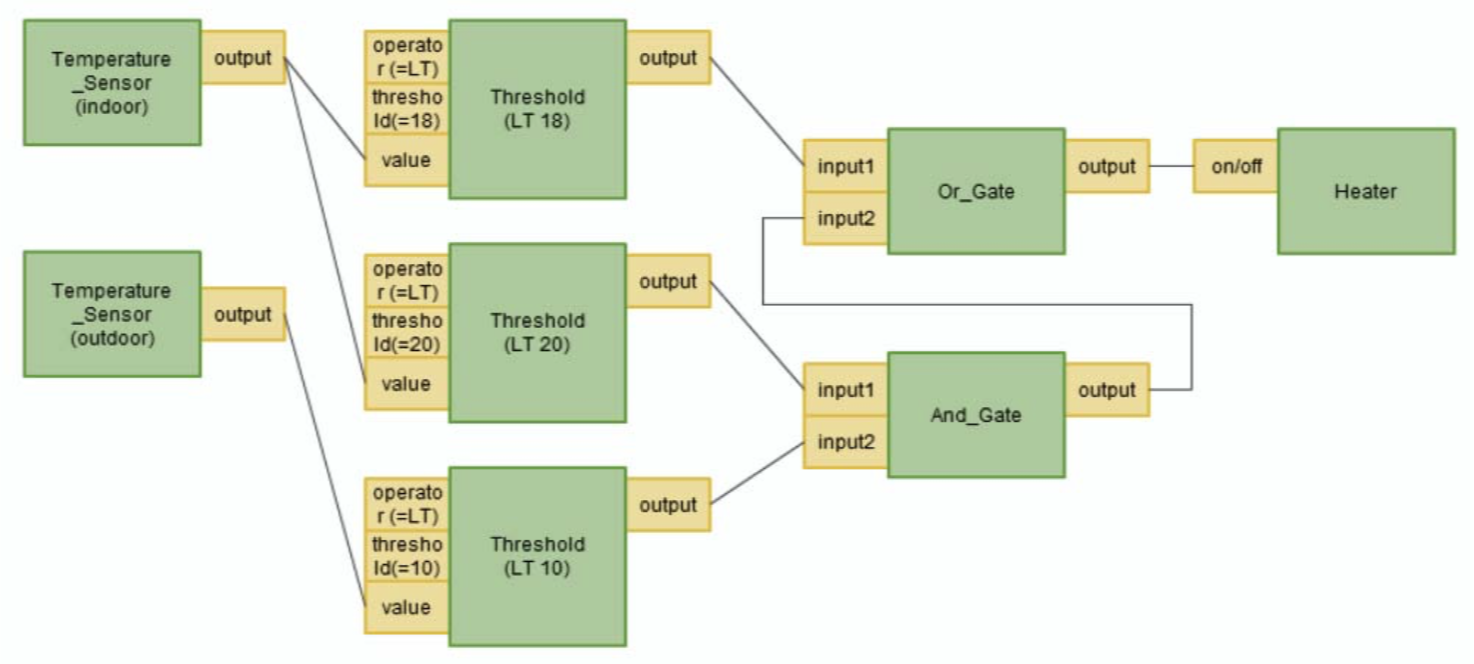
\includegraphics[width=0.8\linewidth]{wukong-fbp.png}
  \caption{Example WuKong flow based programme}
  \label{fig-wukong-fbp}
\end{figure}


Applications in WuKong are written in the form of a flow based programme, an example of which is shown in Figure \ref{fig-wukong-fbp}. Components are called WuObjects, and are instances of WuClasses. Each WuClass has a number of input and output properties. For example, the Temperature Sensor WuClass has a single 'output' property, while the Heater has a single 'on/off' property.

When deploying an application, the host, called 'master' in WuKong, will first discover the available resources in the network and then try to find a node to deploy each component on.

For a node's hardware components, the node creates WuObjects to represent them at startup, so the master can discover the sensors and actuators available in the network. When deploying the application, the master may use a hardware WuObject by connecting its properties.

Software components, like the Threshold or And\_Gate in the example, can be written in either C or Java. A node may have native C implementations built in for a number of commonly used classes from the WuKong standard library, which it will advertise during the discovery phase. If the master cannot find a native implementation of a required class, it may use a Java version instead, which is slower, but more flexible since it can be deployed as part of the application. To support this, the WuKong middleware contains a version of the Darjeeling JVM \cite{Brouwers:2009cj}.

An WuClass is defined by  and two C functions or Java methods:
\begin{itemize}
	\item Its list of properties
	\item A \mycode{setup()} function, called once when an object is created
	\item A \mycode{update()} function, called (i) periodically, for example to sample a sensor, or (ii) when one of the input properties changes value, to compute a new output value or drive an actuator
\end{itemize}

The WuKong middleware takes care of propagating property changes along the links drawn in the FBP. For example, if in Figure \ref{fig-wukong-fbp} the output of the Or\_Gate changes, the new output value is automatically propagated to the Heater's on/off property, and the Heater's \mycode{update()} function is called. An application in WuKong is defined by a number of compact tables, describing the components and links between them, and optionally a number of Java WuClasses.

In WuKong's vision, the master dynamically manages the network. A node may be used in multiple applications, and it's tasks may change dynamically while the application is running if the master decides to reconfigure the network, for example in response to failure \cite{Su:2014uf} or because network conditions change.


\section{Sensor node virtual machines}
Many VMs have been proposed that are small enough to fit on a resource-constrained sensor node. They can be divided into two categories: generic VMs and application-specific VMs, or ASVMs \cite{Culler05} that provide specialised instructions for a specific problem domain. As an example, designed specifically for WSN, Mat\'e \cite{Levis:2002ku} was one of the first to prove VMs can be made to run on sensor nodes. It provides single instructions for tasks that are common on a sensor node, so programmes can be very short.  

SwissQM \cite{Muller:2007fs} is a more traditional and more powerful VM, based on a subset of the Java VM, but extended with sensor network specific instructions to access sensors and do data aggregation. In both systems however, the application has to be programmed in very low level, assembly-like language, limiting their target audience.

VM* \cite{Koshy:2005ww} sits halfway between the generic and ASVM approach. It is a Java VM that can be extended with new features according to application requirements. Unfortunately, it is closed source.

Several generic VMs for high level languages like Python or Java have also been developed, which fit on severely resource constrained nodes. Almost all rewrite the original bytecode to their own format and employ various techniques to reduce code size. Some functionality is sacrificed in order to fit on the sensor nodes, for instance reflection or floating point support are typically not supported.

The Python-on-a-chip project \cite{python-on-a-chip} developed a Python bytecode interpreter small enough to fit on sensor nodes. Requiring 55K of programme memory and a recommended 8K of RAM, it fits on many, but not all of the current sensor boards. MicroPython \cite{micropython} requires slightly more hardware at 256KB programme and 16KB RAM, but has it's own hardware platform and runs Python 3.

The smallest official Java standard is the Connected Device Limited Configuration \cite{CLDC}, but since it targets devices with at least a 16 or 32-bit CPU and 160-512KB of flash memory available, it is still too large for most sensor nodes. The available Java VMs for sensor nodes all offer some subset of the standard Java functionality, occupying different points in the tradeoff between the features they provide, and the resources they require.

Darjeeling \cite{Brouwers:2009cj} from Delft University of Technology is able to run modified Java bytecode on sensor nodes, with only minor restrictions. It has no support for floating point, 64-bit datatypes, reflection or synchronised method calls, although the later is not really a restriction since synchronised blocks are supported. Similarly TakaTuka \cite{Aslam:2008} is a slightly more complete and more complex JVM, also running on both AVR and MSP based sensor nodes and offering it’s own debugger. Another unique property is it's ability to reduce garbage collection cost by static code analysis. Whenever the compiler can determine an object can be safely discarded at a certain point, it annotates the bytecode to tell the VM to do so, thus freeing up memory earlier and reducing the number of times the garbage collector has to run. Sun’s Squawk VM \cite{Shaylor:2003ws} is significantly larger than Darjeeling and TakaTuka, but offers full CLDC compliance.

The opposite approach is taken by NanoVM \cite{Harbaum}, which takes a minimal approach, trading support for a large number of java opcodes for simplicity and code size. The whole VM fits in the 8K flash of an ATMega8 CPU, leaving 512bytes of EEPROM and 75\% of the CPU’s 1K RAM to the application.

Finally, SensorScheme \cite{Evers:2010ur} implements a fully functioning LISP interpreter in under 41KB.

\subsection{Darjeeling}
Since our VM is based on Darjeeling, we will examine it in more detail in this section.

\paragraph{Split VM architecture}
\begin{figure}[H]
	\centering
	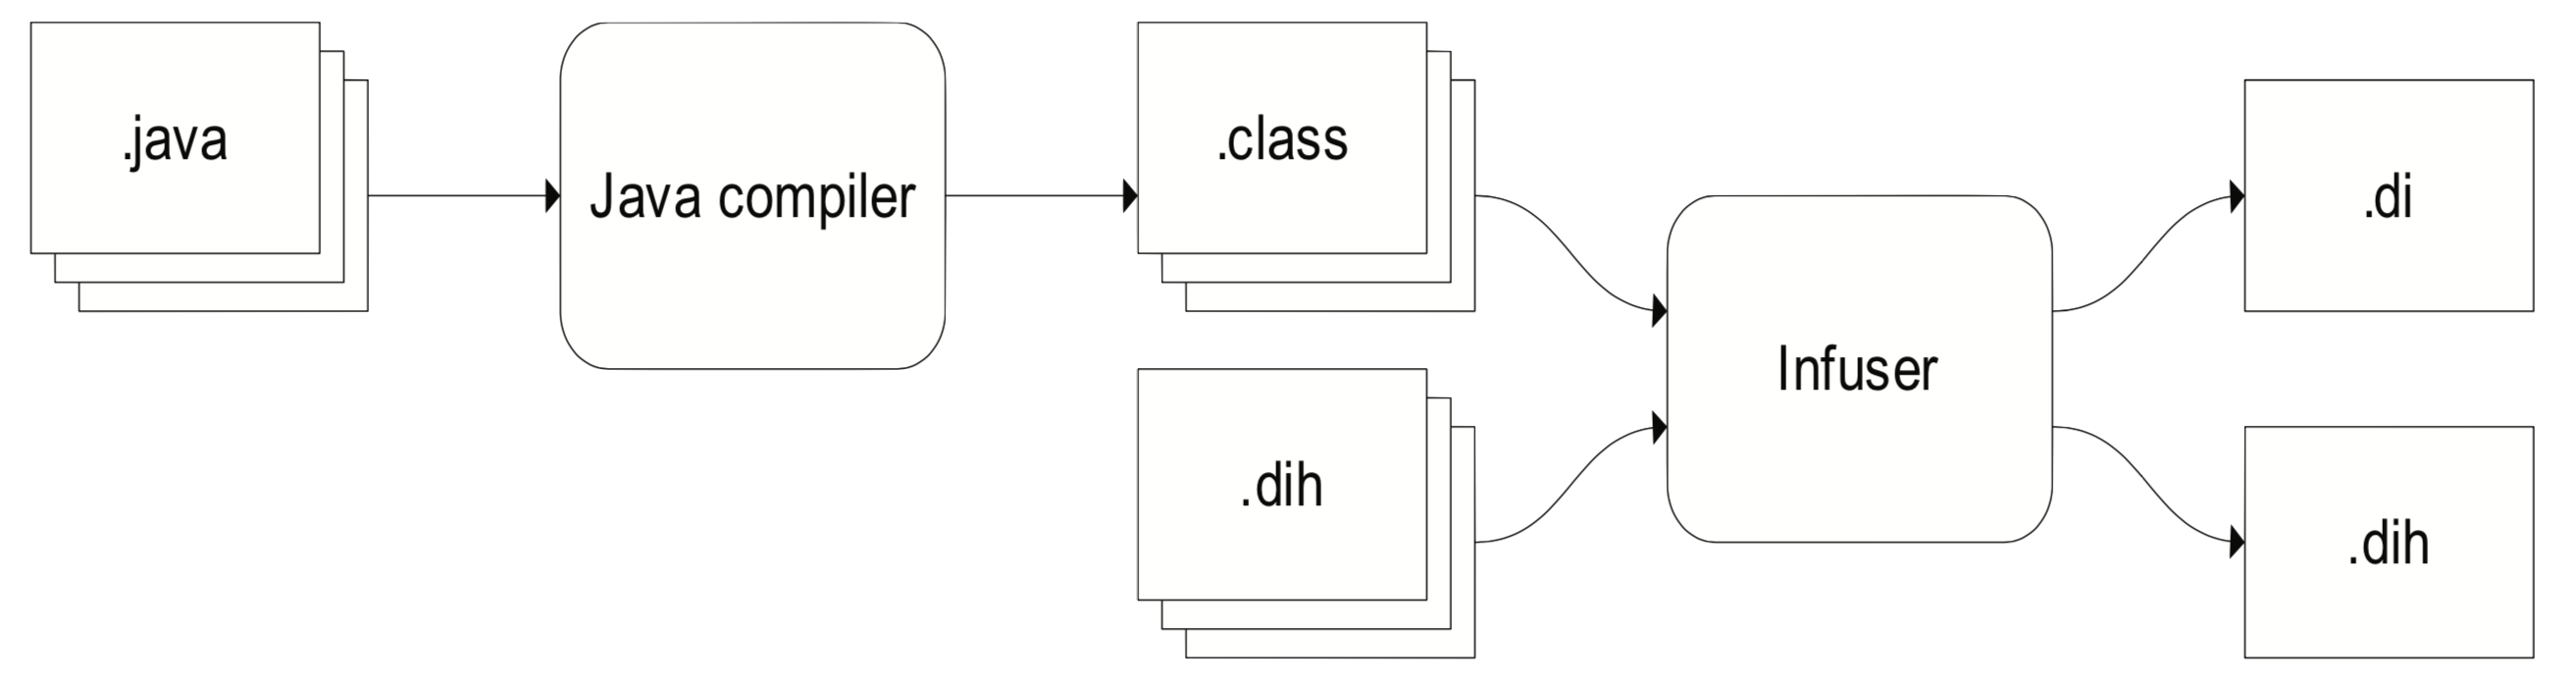
\includegraphics[width=0.6\linewidth]{darjeeling-infusion-process}
	\caption{Darjeeling infusion process, taken from \cite{Brouwers:2009cj}}
	\label{fig-darjeeling-infusion-process}
\end{figure}
Like most other sensor node JVMs, it uses a \emph{split VM architecture} \cite{Simon:2006wd}. The actual virtual machine running on the node does not use standard JVM class files, but these class files first have to be transformed by an offline tool into a format more suitable for a sensor node. In Darjeeling's case this tool is called the \emph{infuser}, which takes several Java classes and statically links them into a single \emph{infusion}.

The infuser changes the bytecode in several ways, replacing named references by a numbering scheme, so that the constant strings with class and method names can be removed from the constant pool, and flattening the Java classes into a list of statically entities. Infusions are typically libraries, such as the \mycode{java.lang} base library, networking protocols, or the application. An infusion can reference code in another infusion using header files, created during the infusion process that allow it to find the numbered identifiers of classes and methods in the referenced infusion. This is shown in Figure \ref{fig-darjeeling-infusion-process}.

\paragraph{16-bit architecture}
\begin{figure}[H]
	\centering
	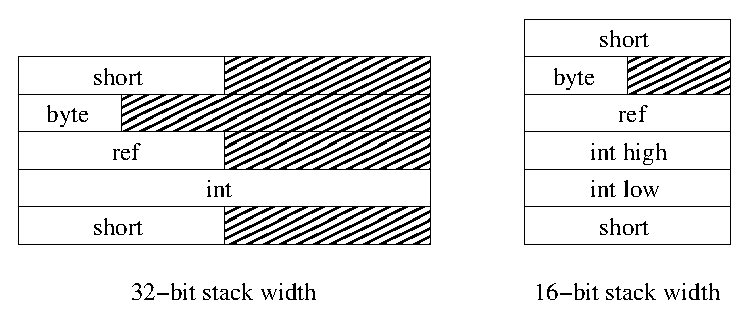
\includegraphics[width=0.6\linewidth]{32bit-vs-16bit-stack}
	\caption{Unused memory for 32 and 16-bit stack width}
	\label{fig-32bit-vs-16bit-stack}
\end{figure}

Besides statically linking classes, the infuser also makes several changes to the bytecode format. Since references on sensor nodes are usually 16-bit, and the use of 8-bit and 16-bit integer variable are commonly used in sensor node code to save memory, storing all data in 32-bit slots as the JVM does would lead to significant overhead, as shown in Figure \ref{fig-32bit-vs-16bit-stack}. Therefore, Darjeeling stack and variable slots are 16-bit wide, using two slots for 32-bit ints, similar to how the normal JVM uses two 32-bit slots for 64-bit longs. This means Darjeeling's bytecode also introduces 16-bit versions of many opcodes, for example \mycode{SADD} adds two 16-bit shorts, while \mycode{IADD} adds two 32-bit ints. The infuser analyses the type of expressions, and replaces the 32-bit instructions found in normal JVM bytecode with the 16-bit variants where possible.



\paragraph{Double-ended stack}
\begin{figure}[H]
	\centering
	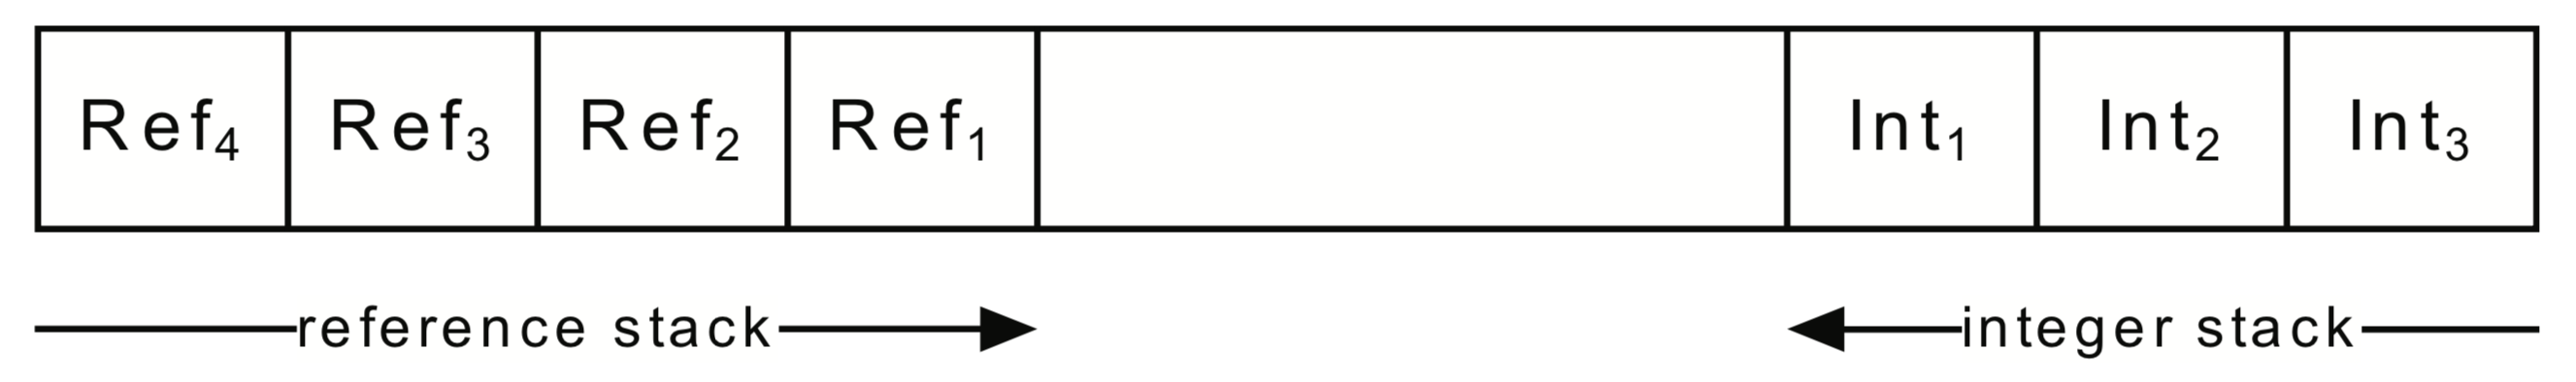
\includegraphics[width=0.6\linewidth]{darjeeling-split-stack}
	\caption{Darjeeling split operand stack, taken from \cite{Brouwers:2009cj}}
	\label{fig-darjeeling-split-stack}
\end{figure}

A second important modification is that Darjeeling splits the operand stack into separate reference and integer stacks, as shown in Figure \ref{fig-darjeeling-split-stack}. Each stack frame still allocates the same amount of space for it's operand stack, but Darjeeling places references on one side, and integers on the other. At the expense of having to keep track of two operand stack pointer, this reduces the complexity of the garbage collector significantly. When the garbage collector runs, it needs to find the \emph{root set} of all live objects, which includes objects with references on the stack but not stored elsewhere. Since the type of the values on the operand stack changes continuously, it would be hard to determine which values are references and which are integers in a single stack, but using Darjeeling's split stack design, it can simply place all values on the reference stack in the root set. For the same reason, Darjeeling also groups the slots allocated for local, static and instance variables into an integer and reference group.

The necessary modifications to the byte code are taken care of by the infuser. Generic stack instructions such as \mycode{pop} are replaced by distinct versions for the integer and reference stack: \mycode{ipop} and \mycode{apop}.

\paragraph{Limitations}
Darjeeling implements a significant subset of Java, but like all sensor node JVMs needs to make some sacrifices to scale down to sensor node size. Specifically, it does not support the 64-bit \mycode{long} datatype or floating point variables. It does not support reflection, since the infusion process drops the necessary type information from its class files to significantly reduce their size. And it does not support the \mycode{synchronized} modifier on static methods.

\section{Performance}
While many different VMs have been published, only a few papers describing sensor node VMs contain detailed performance measurements, shown earlier in Table \ref{tbl-slowdown-for-sensornode-vms}. Darjeeling \cite{Brouwers:2009cj} reports between 30x and 113x slowdown for 3 benchmarks in 16-bit and 32-bit variations, compared to the native C equivalent. Ellul \cite{Ellul:2012thesis} reports measurements on the TakaTuka VM \cite{Aslam:2008} where the VM is 230x slower than native code, and consumes 150x as much energy. TinyVM \cite{Hong:2009gc} is between 14x and 72x slower than C, for a set of 9 benchmarks. DVM \cite{Balani:2006} has different versions of the same benchmark, where the fully interpreted version is 108x slower than the fully native version. Finally, SensorScheme \cite{Evers:2010ur} is up to 105x slower. Since performance depends on many factors, it is hard to compare these numbers directly. But the general picture is clear: current interpreters are one to two orders of magnitude slower than native code.

Translating bytecode to native code to improve performance has been a common practice for many years. A wide body of work exists exploring various approaches, either offline, ahead-of-time  or just-in-time. One common offline method is to first translate the Java code to C as an intermediate language, and take advantage of the high quality C compilers available \cite{Dean:1996wb, Muller:1997}. Courbot et al. describe a different approach, where code size is reduced by partly running the application before it is loaded onto the node, allowing them to eliminate code that is only needed during initialisation \cite{Courbot:2010}. Although the initialised objects are translated to C structures that are compiled and linked into a single image, the bytecode is still interpreted. While in general we can produce higher quality code when compiling offline, doing so sacrifices key advantages of using a VM.

Hsieh et al. describe an early ahead-of-time compiling desktop Java VM \cite{Hsieh:1996cy}, focussing on translating the JVM's stack-based architecture to a register based one. In the Japale\~no VM, Alpern et al. take an approach that holds somewhere between AOT and JIT compilation \cite{Alpern:1999}. The VM compiles all code to native code before execution, but can choose from two different compilers to do so. A fast baseline compiler simply mimics the Java stack, but either before or during run-time, a slower optimising compiler may be used to speed up critical methods.

Since JIT compilers work at run-time, much effort has gone into making the compilation process as light weight as possible, for example \cite{Krall:1998}. More recently these efforts have included JIT compilers targeted specifically at embedded devices. Swift \cite{Zhang:2012wf} is a light-weight JVM that improves performance by translating a register-based bytecode to native code. But while the Android devices targeted by Swift may be considered embedded devices, they are still quite powerful and the transformations Swift does are too complex for the ATmega class of devices. HotPathVM \cite{Gal:2006} has lower requirements, but at 150KB for both code and data, this is still an order of magnitude above our target devices.

Given our extreme size constraints - ideally we only want to use in the order of 100 bytes of RAM to allow our approach to be useful on a broad range of devices, and leave ample space for other tasks on the device - almost all AOT and JIT techniques found in literature require too much resources. Indeed, some authors suggest sensor nodes are too restricted to make AOT or JIT compilation feasible \cite{Aslam:2011thesis, Wirjawan:2008}.

\subsection{AOT compilation for sensor nodes}
\label{sec-state-of-the-art-elluls-aot}
% NOTE: the 811\% here comes from the manual optimisation table. since we calculate overhead slightly different there to be able to split it into 3 components, the total in that table is 811 instead of 815 in the trace output text file.
On the desktop, VM performance has been studied extensively, but for sensor node VMs this aspect has been mostly ignored. To the best of our knowledge AOT compilation on a sensor node has only been tried by Ellul and Martinez \cite{Ellul:2010iw, Ellul:2012thesis}, and our work builds on their approach.

Their approach is both simple and effective. To translate JVM bytecode each JVM bytecode instruction is simply replaced by a fixed sequence of native instructions that implement it. This can be done in a single pass, as the bytecode is being received by the node, writing native code to flash memory instead of the JVM bytecode. Like Darjeeling, they use a split stack architecture, with the CPU's native stack doubling as integer operand stack for each access, while reference operands are still stored in the stack frame.

\begin{table}[]
\centering
\caption{Example of Ellul's Bytecode to Native Code Translation of \mycode{c=a+b;}}
\label{tbl-ellul-aot-example}
\begin{tabular}{llll}
\toprule
Bytecode           & Stack before        & Stack after         & Native pseudo assembly code \\
\midrule
\mycode{ILOAD\_0}  & ...                 & ...                 & \mycode{LOAD r1, a} \\
                   & ...                 & ..., value1         & \mycode{PUSH r1} \\
\mycode{ILOAD\_1}  & ..., value1         & ..., value1         & \mycode{LOAD r1, b} \\
                   & ..., value1         & ..., value1, value2 & \mycode{PUSH r1} \\
\mycode{IADD}      & ..., value1, value2 & ..., value1         & \mycode{POP r1} \\
                   & ..., value1         & ...                 & \mycode{POP r2} \\
                   & ...                 & ...                 & \mycode{ADD r1, r2} \\
                   & ...                 & ..., result         & \mycode{PUSH r1} \\
\mycode{ISTORE\_2} & ..., result         & ...                 & \mycode{POP r1} \\
                   & ...                 & ...                 & \mycode{STORE c, r1} \\
\bottomrule
\end{tabular}
\end{table}

Table \ref{tbl-ellul-aot-example} shows how a simple statement is translated to native code. The blocks each JVM bytecode instruction translates to are fixed. This simple translation to native code removes the interpreter loop, which is by far the biggest source of overhead in interpreting VMs, but it is clear from the native pseudo code in Table \ref{tbl-ellul-aot-example} that this approach results in many unnecessary push and pop instructions. Since the JVM is a stack-based VM, each instruction first obtains its operands from the stack and pushes any result back onto it. As a result, over half the instructions are push or pop instructions.

\subsubsection{Peephole optimisation}
To reduce this overhead, Ellul proposes a simple peephole optimiser \cite{Ellul:2012thesis} which does 4 optimisation, for each which an examples is shown in Table \ref{tbl-ellul-peephole}. The most important are removing a push immediately followed by a pop to the same register, since this has no net effect. If the source and destination registers differ, the two instructions are replaced by a move. Note that the assembly code shown here is for the MSP430 CPU.

\begin{table}[]
\centering
\caption{Ellul's peephole optimisations}
\label{tbl-ellul-peephole}
\begin{threeparttable}
\begin{tabular}{lrrlrr}
\toprule
Before &  &  & After &  & \\
Instructions      & Cycles & Length & Instructions      & Cycles & Length \\
\midrule
\midrule
PUSH R13          & 6      & 2      &                   & 0      & 0 \\
POP R13           &        &        &                   &        & \\
\midrule
PUSH R13          & 6      & 2      & MOV R13, R14      & 1      & 1 \\
POP R14           &        &        &                   &        & \\
\midrule
MOV \#0, R15      & 2      & 2      & CLR R15           & 2      & 1 \\
\midrule
MOV R6,R5         & 5      & 3      & MOV R6,0x0000(R4) & 4      & 2 \\
MOV R5,0x0000(R4) &        &        &                   &        & \\
\bottomrule
\end{tabular}
\begin{tablenotes}
\item MSP430 assembly, taken from \cite{Ellul:2012thesis}
\end{tablenotes}
\end{threeparttable}
\end{table}

% TODO: read \cite{Suganuma:2000vl} and possibly quote for stack technique, see Joshua p. 59

\subsubsection{Resulting performance}
Ellul's approach improves performance considerably compared to the interpreters, but using the standard CoreMark benchmark \cite{coremark}, it still generates code that is still up to 9x slower than optimised native C. The average slowdown found in our benchmarks was 5.4x.

It is important to further improve this for two reasons. First, even if an application is asleep for a large percentage of the time, it may at times want to measure something at high resolution, similar to how ADAE \cite{Chang:2010ek} responds to what it calls 'interesting events' by taking extra measurements as long as its energy budget permits. Any slowdown in the VM will affect the maximum rate at which such samples can be taken.

Second, reduced performance means the CPU has to stay active for a longer time, resulting in increased cpu power consumption and reduced battery life. If we look back to the data in Section \ref{sec-introduction-performance}, we see in Table \ref{tbl-mercury-energy} that the 'Computer features' optimisation, which reduces the amount of data to be transmitted by over 98\% is still a net gain, even if a 8x slowdown would mean it takes 6462uJ to compute the features. However it makes the CPU a large energy consumer which would affect battery life if the application didn't use such an expensive sensor as a gyro. Looking at the FFT, this is already a major energy consumer, and would become the largest one at only 4.1x slowdown.

Looking at the calculations for lossless compression, also in Section \ref{sec-introduction-performance}, we saw that in this particular case, the ratio of the energy saved on radio transmission vs energy spent on compression was about 1.9:1. This result depends on many factors, for instance less than ideal network conditions may cause retransmissions, increasing the cost per bit sent and making compression more worthwhile. However in this particular case the slowdown incurred even after Ellul's optimisation would make compression a net loss. Any slowdown push some situations past the break-even point, or reduces the benefits of compression in others.

Regardless of these concerns, there are scenarios that may not be able to tolerate the one to two orders of magnitude slowdown seen in interpreters, a slowdown of up to 9x for Ellul's AOT approach may be acceptable. However, there is a second reason to want to improve on it, which is it also results in significantly larger code: on average 2.8x larger. This reduces the amount of code we can load onto a node, and given that flash memory is already restricted, this is a major sacrifice to make when adopting AOT on sensor nodes.


\section{Safety}
\label{sec-state-of-the-art-safety}
With some exceptions \cite{Evers:2010ur}, most current sensor node VMs don't discuss safety, but instead focus on the functionality provided and how this can be implemented on a tiny sensor node. This is unfortunate, because the ability to provide a safety execution environment is both desirable, and easier to implement using a VM than it is using native code.

Several non-VM systems exists to provide various levels of safety for sensor nodes. They fall into two distinct categories: they either depend on a trusted host to add the necessary checks, or they allow the node to guarantee safety independent of whatever code it may receive from the host. The first protects against programming errors, while the latter can protect against malicious attacks. Obviously the latter is the stronger guarantee, but it also comes at a higher price.

\subsection{Source code approaches}
In the first category are systems that guarantee safety at the source code level. Virgil \cite{Titzer:2006uy} is a language that is inherently safe and specifically designed for sensor nodes. The application is explicitly split into an initialisation and run-time phase, where objects are only allocated during the initialisation phase. The initialisation phase happens during compilation (to C code), which means all object and their locations are know at this point, allowing Virgil to ensure safety and optimise the code at compile time.

Safe TinyOS on the other hand, works on annotated nesC TinyOS code. It uses the Deputy \cite{Condit:2007uo} source-to-source compiler to analyse the C source code and insert the necessary run-time checks were necessary. Because this happens on the host, before sending the code to the node, it can use the host's resources to do more complex analysis of the source code and eliminate checks where the it can determine a memory access to be safe at compile time, resulting in a much lower overhead

Both approaches eventually result in standard C, which is then compiled and sent to the node. Therefore, both approaches may protect against accidental programming errors, but not against malicious code an attacker may send to it.

\subsection{Native code approaches}
For desktop applications, Wahbe et al. described software fault isolation \cite{Wahbe:1994cj} techniques to isolate a piece of untrusted code, without the overhead of using processes and the CPU's memory protection. A typical example is a plugin that frequently needs to interact with an application. It should be isolated from the application so bugs in the plugin can't bring down the whole application, but running it as a separate process would incur high overhead due to frequent context switches. Two basic methods are described to isolate such code from the main application: we can either rewrite the native code at load time, inserting checks at all potentially unsafe writes, or we can compile the code to a more restricted format with the appropriate checks already in place, and verify the code adheres to this standard at load time.

Since we don't have processes or CPU memory protection on a sensor node, Wahbe's approach provides an attractive alternative. Two systems exist that provide safety for sensor nodes using each of these approaches.

\emph{t-kernel} does more than providing memory safety. It raises the level of system abstraction for the developer by providing three features typically missing on sensor nodes: preemptive scheduling, virtual memory, and memory protection. It does this by extensive rewriting of the binary code at load time. While \emph{t-kernel} is heavily optimised, the price for this is that programmes still run 50-200\% slower, and code size increases by 500-750\%.

The other approach is taken by Harbor \cite{Kumar:2007ge}, which consists of two components. On the desktop a binary rewriter sandboxes an application by inserting run-time checks before it is sent to the node. The SOS operating system \cite{Han:2005th} is then extended with a binary verifier to verify incoming binaries. The correctness only depends on the correctness of this verifier. The increase in code size is more modest than for \emph{t-kernel} at a 30-65\% increase, but performance is 160-1230\% slower, where the authors note the benchmark producing the highest slowdown is more typical of sensor node code. They also note more complex analysis of the binary code could reduce the number of necessary checks, but at the cost of significantly increasing the complexity of the verifier.

